\begin{table*}[t]
	\small
	\centering
	\caption{RMSE (M) / RPE (M/S) of 3 VO algorithms in slo-mo/normal speed on Selected Sequences}
	\begin{tabular}{c|c||c|c|c||c|c|c|c|c}
		\toprule[1pt]
		\midrule[0.1pt]
		\textbf{ } & 
		& \multicolumn{3}{c||}{\bfseries \small one run in \textit{slo-mo}}
		& \multicolumn{5}{c}{\bfseries \small five runs in normal speed (\#failures are highlighted by -/\textcolor{f4}{4}/\textcolor{f3}{3}/\textcolor{f2}{2}/\textcolor{f1}{1}/0)} \\
		\cmidrule{3-10}
		& \textbf{\small Seq.} & SVO\cite{SVO2017} & DSO\cite{DSO2017} & ORB\cite{ORBSLAM}  & SVO\cite{SVO2017} & DSO\cite{DSO2017} & ORB\cite{ORBSLAM} & GF-ORB\cite{zhao2018good2} & MH-ORB\cite{zhao2019maphash} \\
		\midrule
		\  \parbox[t]{1mm}{\multirow{8}{*}{\rotatebox[origin=c]{90}{\textbf{RMSE}}}} \ 
				
		& \textit{f2 desk person}  & 1.26e0 	& 1.25e-1	& \underline{4.76e-2}  & \textcolor{f1}{1.53e0}& \textcolor{f0}{5.36e-1}& \textcolor{f0}{5.94e-2} & \textcolor{f0}{3.51e-2} &  \underline{\textcolor{f0}{2.88e-2}}\\
		
		& \textit{lr kt0}			& 4.97e-1	& 2.21e-1	&	\underline{2.10e-1}	 & \textcolor{f0}{3.07e-1} & \underline{\textcolor{f0}{2.61e-1}} & - & - & -			\\		
		
		& \textit{of kt3}			& 6.43e-1	& \underline{3.82e-2}	&	5.58e-2		 &\textcolor{f0}{5.60e-1} & \underline{\textcolor{f0}{3.87e-2}}&\textcolor{f0}{2.57e-1} & \textcolor{f0}{2.76e-1} & 	 \textcolor{f0}{6.69e-2}	\\
		
		& \textit{room3}  			& 2.03e0	& 2.86-1	& \underline{2.09e-1}  & \textcolor{f2}{2.02e0}& - & \underline{\textcolor{f2}{1.80e-1}} & -&  -\\ 		
		
		& \textit{outdoors4}  		& -		 	& \underline{2.21e-2} 	& 8.39e-2  & \underline{\textcolor{f3}{1.74e0}}& - & - & -&  -\\ 
				
		& \textit{MH 05 diff}  		& 4.26e0 	& \underline{1.38e-1}	& 3.03e-1 &  \textcolor{f1}{1.44e0} & \underline{\textcolor{f4}{1.08e-1}}& \textcolor{f0}{1.18e0} & \textcolor{f0}{1.43e-1} & \textcolor{f0}{2.29e-1}\\ 
		
		& \textit{V1 01 diff}  		& 5.53e-1 	& 1.08e0 	& \underline{2.32e-1}  & \textcolor{f0}{6.09e-1} & \textcolor{f0}{1.34e0}& \textcolor{f3}{1.25e0}& \textcolor{f4}{9.23e-1}&  \underline{\textcolor{f2}{4.61e-1}}\\ 
		
		\cline{2-10} 
		\vspace{-1pt}
		& \textbf{Average}  		& 1.54 	& 0.50 	& \underline{0.16}  & 1.17 & 0.46 & 0.59 & 0.34 & \underline{0.20} \\ 
		%
		\midrule
		\  \parbox[t]{1mm}{\multirow{5}{*}{\rotatebox[origin=c]{90}{\textbf{RPE}}}}\ 
				
		& \textit{KITTI Seq 04} 	& 2.06e0 	& \underline{7.88e-2} 	& 9.18e-2  & \textcolor{f0}{1.82e0} & \underline{\textcolor{f0}{8.09e-2}}&\textcolor{f0}{9.74e-2} & \textcolor{f0}{1.00e-1} &  \textcolor{f0}{9.92e-2} \\ 
		
		& \textit{KITTI Seq 02}		& 6.91e0		& \underline{1.31e-1}		& 1.38e-1	 & \textcolor{f0}{7.17e0} & \textcolor{f0}{1.52e-1}& \textcolor{f2}{2.08e-1} & - &  \underline{\textcolor{f3}{1.41e-1}}\\	
		
		& \textit{conf. hall1} 		& 4.35e-1  & \underline{4.33e-1}	& -	 & \textcolor{f0}{4.25e-1}& \textcolor{f0}{4.57e-1}& \underline{\textcolor{f4}{1.50e-1}}& \textcolor{f0}{1.64e-1}& \textcolor{f1}{2.17e-1}\\%\textbf{2.24e-1} \\ 
		
		& \textit{corridor}			& 1.20e0	&	6.50e-1		&	\underline{2.34e-1}	 & \textcolor{f0}{1.38e0}& \underline{\textcolor{f0}{5.31e-1}}& \textcolor{f4}{1.54e0}& \textcolor{f0}{6.22e-1}& \textcolor{f1}{1.05e0}\\
		
		& \textit{NewCollege}  		& -        & 1.92e-2   & \underline{1.65e-2}  & - & \textcolor{f0}{1.93e-2} & \underline{\textcolor{f1}{1.88e-2}}& \textcolor{f0}{1.95e-2}&  \textcolor{f0}{1.92e-2}\\ 	
		%
		\cline{2-10} 
		\vspace{-1pt}
		& \textbf{Average}  		& 2.65 	& 0.26 	& \underline{0.12}  & 2.70 & 0.25 & 0.40 & \underline{0.23} & 0.31 \\ 
		\midrule[0.1pt]
 	\bottomrule	[1pt]
	\end{tabular} 
	\label{tab:accuracy_summary}
\end{table*}



Time profiling of the computational modules of a SLAM system provides
clues to how SLAM implementations should be improved at the
computational component level.  This is particularly true for
feature-based methods, which typically are more costly than direct
methods.
To understand the time consumption of the modules in a SLAM 
pipeline, we advocate fine-grained time profiling and the use of
time-dilation when evaluating SLAM systems with ROS bag playback, i.e.
\textit{slo-mo} playback. 
The idea is similar to the \textit{process-every-frame} mode in 
SLAMBench~\cite{nardi2015introducing}, which continues with the next frame 
after the previous frame is completely processed, The proposed 
\textit{slo-mo} is straightforward and easy to apply in ROS. 
We conjecture that \textit{slo-mo} playback will establish performance 
upper-bounds for evaluated SLAM systems, which serves as a hint on the
potential of SLAM system (e.g. running on better hardware in the near
future).
The time scaling factor for \textit{slo-mo} playback was chosen to be
0.2, providing 5x more time for a single-frame update.

Quantitative eqvaluation on the chosen 12 sequences involved three 
state-of-the-art VO/SLAM algorithms, i.e. SVO~\cite{SVO2017},
DSO~\cite{DSO2017} and ORB-SLAM (ORB)~\cite{ORBSLAM}.  For those using
features, the feature quantity parameter was set to use 800 features 
per frame in \textit{slo-mo}. 
The testbed is a laptop with a Intel Core i7-6820HQ quadcore 2.70GHz 
CPU and 32 GB memory. 
The loop-closure thread in ORB-SLAM was disabled to operate like a
visual odometry (VO) system, though the local mapping thread was not
disabled (it behaves like a short-term loop closure). 
Each sequence was tested once for each SLAM algorithm.
Evaluation varied based on the available ground truth.
For sequences with high-precision 6DoF ground truth 
(e.g. from Motion Capture system), tracking accuracy is evaluated 
with RMSE (m) versus the absolute pose references.  
For sequences with less frequent ground truth signals or with
synthesized ground truth (e.g., using SfM), the RMSE of relative pose error 
(m/s) is used.  The time cost of the major computational components of
the three VO algorithms was recorded.

The timing outcomes for the tested algorithms are shown in
Fig~\ref{fig:latency}, where the estimated time cost for each component 
is computed by averaging over all tracked frames in all selected sequences. 
The methods with direct pose estimation components, SVO and DSO, did not
consume significantly more time. 
Interestingly, DSO ran faster in normal speed, which could due to 
the improved inverse-depth estimation provided by back-end.  
With these minor changes, weak performance points 
in these algorithms should be attributed to algorithm performance limits.
ORB-SLAM consumed more time in \textit{slo-mo} versus normal time for
many of the early components, but less time for the pose optimization
step. Faster convergence of the pose optimization implies better
conditioning of the optimization, better predicted poses, or improved
feature selection or coordinate estimation.
For total time cost, ORB-SLAM take the most time processing each frame,
primarily due to the feature extraction and matching.

Pose tracking performance results for \textit{slo-mo} are listed on 
the left side of Table~\ref{tab:accuracy_summary}. On each sequence, 
the method with the lowest RMSE/RPE is underlined and the failure cases 
with tracking loss over one third of the entire seuqence are discarded 
(marked as dash). 
Considering first track loss only, DSO is the only algorithm to
successfully track all sequences. Furthermore, it has good tracking
accuracy (second to ORB-SLAM). This strong performance suggests that
improvements to DSO will most likely involve additional components or
modifications outside of the core DSO components.
In terms of available tracking accuracy, ORB-SLAM achieves the best
performance with average RMSE of 0.16m and average RPE of 0.12m/s.  
However its timing does not match that of DSO, thus modifications should
prioritize enhancing ORB-SLAM's timing properties.
Though SVO has excellent timing, it has the lowest performance with
regards to track loss and pose tracking accuracy 
(average RMSE of 1.5m and average RPE of 2.65m/s).  
These outcomes indicate that, the \textit{slo-mo} can help understand 
performance properties of SLAM systems. 

\begin{figure}[t]
	\centering
	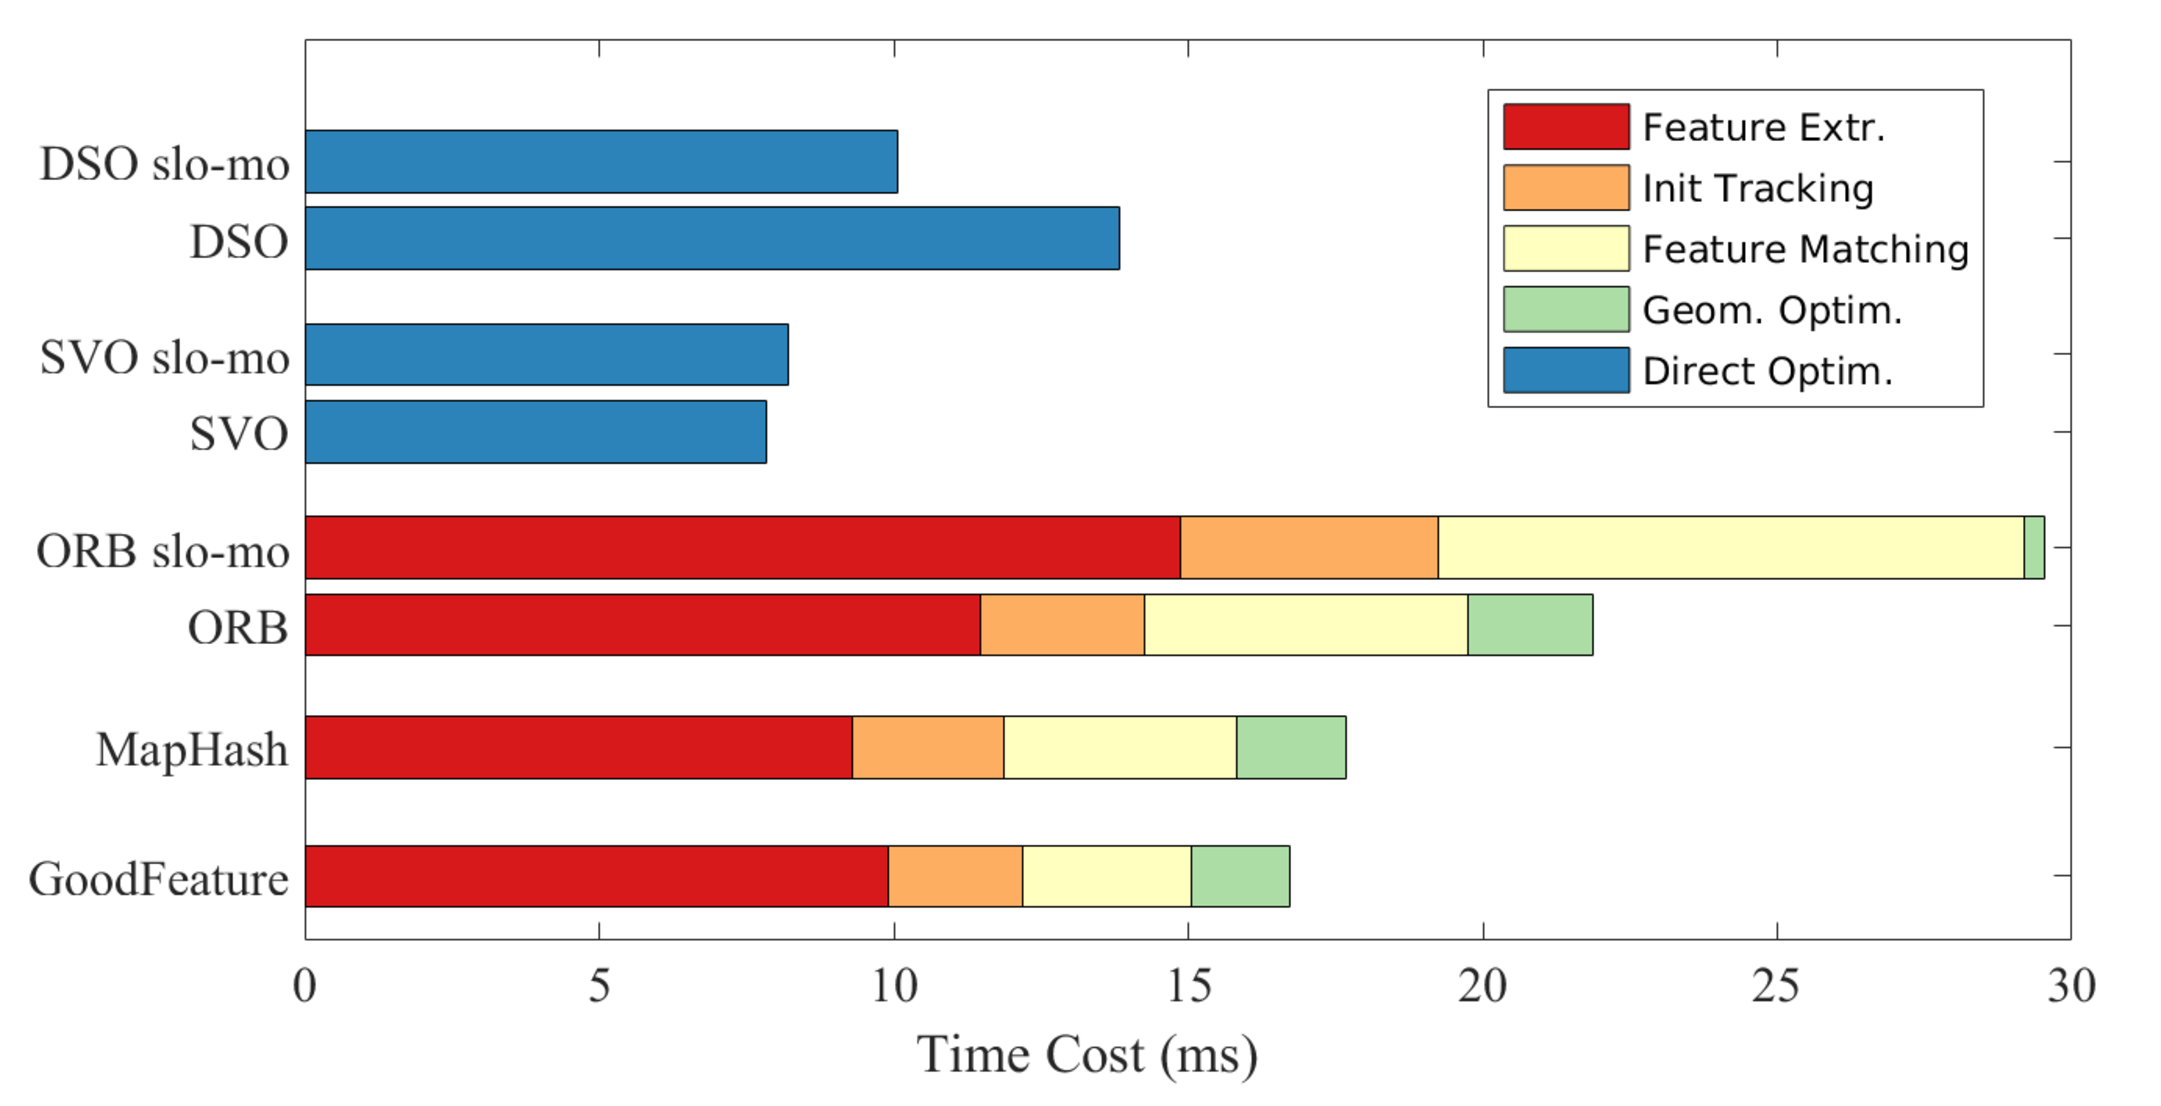
\includegraphics[width=\columnwidth]{./component_timecost.pdf} \\
	\caption{Time profiling of modules in three state-of-the-art VO algorithms and two low-latency algorithms, running under normal speed and \textit{slo-mo}.
 \label{fig:latency}}
\end{figure}





